\documentclass[tikz,convert=false]{standalone}
\begin{document}
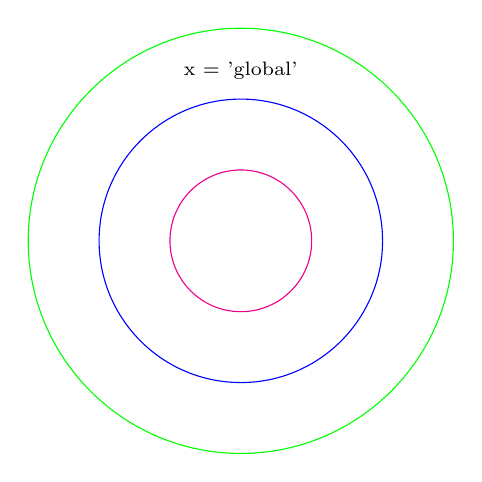
\begin{tikzpicture}[scale=0.6]
\draw [magenta] circle [radius=1.5];
\draw [blue] circle [radius=3];
\node[draw=none,align=center, font=\scriptsize,text width = 1.6cm] at (0,3.6) {x = 'global'};
\draw [green] circle [radius=4.5];
\end{tikzpicture}
\end{document}

\documentclass[tikz,convert=false]{standalone}
\begin{document}
  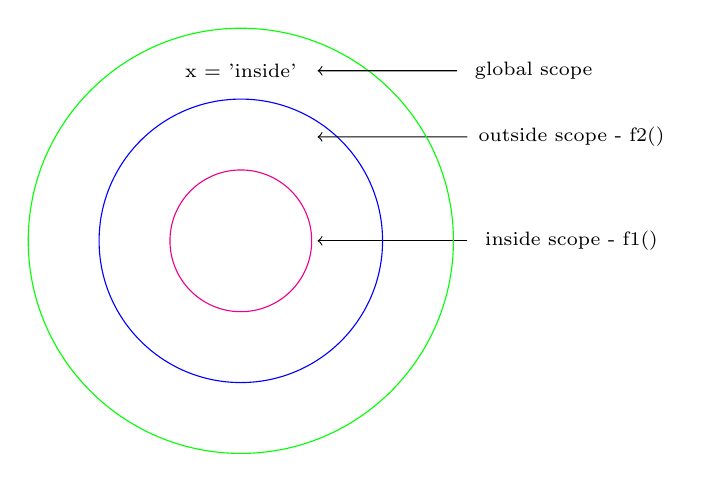
\begin{tikzpicture}[scale=0.6]
    % inside scope
    \draw [magenta] (0,0) circle [radius=1.5] node (i1) {};
    \node [draw=none,align=center, font=\scriptsize,text width = 2.4cm, name=i2] at (7,0) {inside scope - f1()};
    \node[draw=none,align=center, font=\scriptsize,text width = 1.7cm, name=i3] at (0,0) {};
    \draw [->] (i2) -- (i3);

    % outside scope
    \draw [blue] (0,0) circle [radius=3] node (o1) {};
    \node [draw=none,align=center, font=\scriptsize,text width = 2.4cm, name=o2] at (7,2.2) {outside scope - f2()};
    \node[draw=none,align=center, font=\scriptsize,text width = 1.7cm, name=o3] at (0,2.2) {};
    \draw [->] (o2) -- (o3);

    % global scope
    \draw [green] (0,0) circle [radius=4.5]  node (g1) {};
    \node [draw=none,align=center, font=\scriptsize,text width = 1.7cm, name=g2] at (6.2,3.6) {global scope};
    \node [draw=none,align=center, font=\scriptsize,text width = 1.7cm, name=g3] at (0,3.6) {x = 'inside'};
    \draw [->] (g2) -- (g3);
  \end{tikzpicture}
\end{document}